    % Document Class
    \documentclass[12pt,a4paper]{article}

    % Packages essentiels
    \usepackage[utf8]{inputenc}
    \usepackage[T1]{fontenc}
    \usepackage[french]{babel}
    \usepackage{lmodern}

    % Packages mathématiques
    \usepackage{amsmath}
    \usepackage{amssymb}
    \usepackage{amsthm}
    \usepackage{mathtools}

    % Packages pour les graphiques et figures
    \usepackage{graphicx}
    \usepackage{pgfplots}
    \pgfplotsset{compat=1.18}
    \usepackage{float}
    \usepackage{subcaption}

    % Mise en page et design
    \usepackage[hmargin=2.5cm,vmargin=2cm]{geometry}
    \usepackage{fancyhdr}
    \usepackage{enumitem}
    \usepackage{xcolor}
    \usepackage{titlesec}
    \usepackage{siunitx}
    \usepackage{longtable}
    \usepackage{booktabs}
    \usepackage[colorlinks=true,linkcolor=blue,urlcolor=blue,citecolor=blue]{hyperref}

    % Configuration des en-têtes et pieds de page
    \pagestyle{fancy}
    \fancyhf{}
    \fancyhead[L]{\slshape\nouppercase{\leftmark}}
    \fancyhead[R]{\thepage}
    \renewcommand{\headrulewidth}{0.4pt}

    % Définition des environnements mathématiques
    \newtheorem{theorem}{Théorème}[section]
    \newtheorem{proposition}[theorem]{Proposition}
    \newtheorem{lemma}[theorem]{Lemme}
    \newtheorem{corollary}[theorem]{Corollaire}
    \theoremstyle{definition}
    \newtheorem{definition}[theorem]{Définition}
    \newtheorem{example}[theorem]{Exemple}
    \theoremstyle{remark}
    \newtheorem{remark}[theorem]{Remarque}

    % Configuration des titres de sections
    \titleformat{\section}
    {\normalfont\Large\bfseries}{\thesection}{1em}{}
    \titlespacing*{\section}{0pt}{3.5ex plus 1ex minus .2ex}{2.3ex plus .2ex}

    % Informations du document
    \title{\huge\textbf{Impact des news dans les Limit Order Book}}
    \author{LAFERTE Edouard \and AIAD Janis}
    \date{Juin 2024}

    \begin{document}
    \begin{titlepage}
        \begin{center}
            \vspace*{2cm}
            
            \includegraphics[width=0.4\textwidth]{École_polytechnique_signature.png}
            

            
            {\huge\bfseries Impact des news dans les\\[0.4cm] 
            Limit Order Books\par}
            
            \vspace{2cm}
            
            {\Large\textsc{Mémoire de Recherche}\par}
            \vspace{1cm}
            
            {\large
            \begin{tabular}{c}
                \textbf{ROUSSELLE Felix-William}\\[0.2cm]
                \textbf{DEBA Ayouba}\\[0.2cm]
                \textbf{AIAD Janis}
            \end{tabular}\par}
            
            \vspace{1.5cm}
            
            {\large Sous la direction de\par}
            \vspace{0.4cm}
            {\large\textbf{LEHALLE Charles-Albert}\par}
            
            \vfill
            
            {\large Département de Mathématiques Appliquées\\
            École Polytechnique\\[0.4cm]
            Juin 2024\par}
        \end{center}
    \end{titlepage}

    % Page blanche après la page de titre
    \newpage
    \null
    \thispagestyle{empty}
    \newpage

    \begin{abstract}
    \thispagestyle{empty}
    \vspace*{1cm}
    \begin{center}

    \end{center}
    \vspace{1cm}

    Ce mémoire étudie l'impact des news et actualités sur la dynamique des Limit Order Books dans les marchés financiers à haute fréquence. Nous analysons comment les événements d'actualité influencent la microstructure du marché et modifient les comportements des acteurs. Notre approche combine une modélisation mathématique rigoureuse via le modèle Queue Reactive avec une analyse empirique des données de marché.

    \vspace{1cm}
    \textbf{Mots-clés :} Limit Order Book, Trading Haute Fréquence, Modèle Queue Reactive, Impact des News, Microstructure de Marché

\end{abstract}
    \newpage
    \tableofcontents
    \thispagestyle{empty}

    \newpage
    \setcounter{page}{1}
    
    
\section{Données utilisées}
Dans la suite de notre étude, nous étudierons tout particulièrement les actifs GOOGL, LCID, et KHC. Ces actifs correspondent respectivement à Google, Lucid Group Inc (constructeur américain de véhicules électriques de luxe) et The Kraft Heinz Company (multinationale américaine spécialisée dans l'agroalimentaire).

\begin{table}[h!]
\centering
\begin{tabular}{|c|c|c|c|c|c|}
\hline
\textbf{Actif}& \textbf{Nb Timestamps} & \textbf{Nb Add} & \textbf{Nb Cancel} & \textbf{Nb Order} & \textbf{Mean Arrival (ms)}\\ \hline
GOOGL  & 86386103         & 81146187        & 6448095    & 173980437  & \phantom{000} \\ 
\hline
LCID       & 2101840         & 1975378         & 522436  & 4599687  & \phantom{000} \\
\hline
KHC   & 6300128   & 5982598 & 909555 & 13192289  & \phantom{000}                   
\\ \hline
\end{tabular}
\caption{Tableau des données du Nasdaq sur 65 jours du 28 juillet au 4 novembre}
\label{tab:exemple}
\end{table}
\begin{table}[h!]
\centering
\begin{tabular}{|c|c|c|c|c|}
\hline
\textbf{Actif}& \textbf{Nb/Jour Actions}& \textbf{Pct Add} & \textbf{Pct Cancel} & \textbf{Pct Order}\\ \hline
GOOGL & 2676622 & 49,65\%  & 46,64\%     & 3,70\%    \\ 
\hline
LCID  & 70764   & 45,69\%  & 42,94\%    &11,35\%    \\
\hline
KHC  & 202958   & 47,75\%  & 45,34\%  & 6,89\%                     
\\ \hline
\end{tabular}
\caption{Tableau des données du Nasdaq moyennées sur 65 jours}
\label{tab:exemple}
\end{table}
Les données sont issus de la base de données Databento et ne concernent que la bourse du Nasdaq. On voit tout d'abord que certains actifs sont plus tradés que d'autres notamment GOOGL par rapport au deux autres. Les estimations seront donc naturellement plus précise pour cet actif.
\\
\\
Les données sont sous format de dataframe par journée comprenant toutes les modifications apportées au MBO des trois actifs étudiés. Ce MBO comprend alors:
\begin{itemize}
    \item ts\_recv: timestamp du serveur 
    \item ts\_event: timestamp de l'événement     
    \item rtype: type d'événement     
    \item publisher\_id: id du publisher du MBO (2 pour Nasdaq,...)
    \item instrument\_id: id de l'actif sur les marchés
    \item action: Add(A), Cancel(C), Trade(T)
    \item side: Ask(A), Bid(B)
    \item depth: limite considéree
    \item price: prix
    \item size: taille de l'action réalisée
    \item ts\_in\_delta: temps entre le serveur et l'action
    \item sequence: id de l'action propre à l'actif sur les marchés
    \item bid\_px\_0x: prix à la limite x côté bid
    \item ask\_px\_0x: prix à la limite x côté ask
    \item bid\_sz\_0x: taille de la file d'attente à la limite x côté bid
    \item ask\_sz\_0x: taille de la file d'attente à la limite x côté ask
    \item symbol: symbole de l'actif
\end{itemize}


\section{Modélisation de Hurst et extraction de la volatilité}

\subsection{Présentation du modèle de Hurst}

L'exposant de Hurst, noté H, est un indicateur statistique qui permet de caractériser la nature d'une série temporelle, notamment en termes de persistance ou d'anti-persistance. Dans le contexte des marchés financiers haute fréquence, cet exposant nous permet d'analyser la mémoire du processus de prix et de quantifier sa prédictibilité à différentes échelles de temps.

Pour une série temporelle \(X(t)\), l'exposant de Hurst H est défini par la relation:

\[
E[|X(t+\tau) - X(t)|^2] \propto \tau^{2H}
\]

où \(\tau\) représente l'intervalle de temps considéré. L'interprétation de H est la suivante:
\begin{itemize}
    \item H = 0.5 : Le processus est un mouvement brownien standard (marche aléatoire)
    \item H > 0.5 : Le processus présente de la persistance (tendance à maintenir sa direction)
    \item H < 0.5 : Le processus présente de l'anti-persistance (tendance à s'inverser)
\end{itemize}

\subsection{Procédure d'extraction de la volatilité}

Pour extraire la volatilité du processus de prix, nous avons suivi une approche systématique basée sur différentes échelles temporelles. Notre procédure se décompose en plusieurs étapes:

\begin{enumerate}
    \item Calcul du temps moyen entre les changements de prix (\(\Delta t_{avg}\))
    \item Échantillonnage du processus de prix à différentes échelles temporelles:
    \[\{\Delta t_{avg}, 5\Delta t_{avg}, 10\Delta t_{avg}, ..., 3000\Delta t_{avg}\}\]
    \item Pour chaque échelle \(\tau\), calcul des variations de prix normalisées:
    \[\Delta P_{\tau} = \frac{P(t+\tau) - P(t)}{\sigma}\]
    où \(\sigma\) est la moyenne du spread bid-ask
    \item Estimation de la volatilité selon le modèle de Bachelier:
    \[\sigma_{\tau} = \frac{|\Delta P_{\tau}|}{\sqrt{\tau}}\]
\end{enumerate}

\subsection{Résultats empiriques}

L'analyse des données pour l'actif WBD révèle plusieurs caractéristiques intéressantes:

\begin{itemize}
    \item Le temps moyen entre les changements de prix est de l'ordre de \(10^{-3}\) secondes
    \item La distribution des temps d'arrivée présente une queue lourde, caractéristique des processus de Poisson inhomogènes
    \item La volatilité normalisée \(\sigma_{\tau}\) montre une dépendance en loi de puissance par rapport à l'échelle de temps \(\tau\)
\end{itemize}

Notre analyse approfondie de l'exposant de Hurst à différentes échelles temporelles révèle une caractéristique remarquable : contrairement à l'hypothèse classique d'un H ≈ 0.5 pour les marchés efficients, nous observons un H systématiquement inférieur à 0.5, indiquant une forte anti-persistance dans le processus de prix. Ce phénomène est particulièrement prononcé aux échelles microscopiques.

\begin{table}[h!]
\centering
\begin{tabular}{|c|c|}
\hline
\textbf{Échelle temporelle (µs)} & \textbf{Exposant de Hurst (H)} \\
\hline
2 041 & 0.229 \\
10 207 & 0.250 \\
20 415 & 0.268 \\
61 247 & 0.270 \\
204 157 & 0.284 \\
2 041 576 & 0.285 \\
6 124 728 & 0.297 \\
20 415 762 & 0.278 \\
61 247 288 & 0.310 \\
204 157 627 & 0.329 \\
612 472 883 & 0.206 \\
\hline
\end{tabular}
\caption{Estimations de l'exposant de Hurst pour WBD à différentes échelles temporelles}
\label{tab:hurst_exponents}
\end{table}

Cette anti-persistance (H < 0.5) suggère une forte tendance à la réversion vers la moyenne à court terme, caractéristique des marchés dominés par des market makers et des stratégies de trading haute fréquence. Plusieurs observations importantes émergent :

\begin{itemize}
    \item À l'échelle microscopique (< 100 ms), H ≈ 0.23-0.27, indiquant une forte anti-persistance
    \item Aux échelles intermédiaires (100 ms - 60 s), H augmente progressivement jusqu'à ≈ 0.33
    \item Aux échelles plus longues (> 10 min), H diminue à nouveau (≈ 0.21)
\end{itemize}

Cette structure multi-échelle de l'exposant de Hurst reflète différents régimes de marchés et acteurs :
\begin{itemize}
    \item L'anti-persistance à très court terme est cohérente avec le comportement de rebond des prix autour du spread bid-ask
    \item L'augmentation de H aux échelles intermédiaires suggère l'influence croissante des tendances directionnelles
    \item La diminution de H aux échelles plus longues pourrait résulter de l'interaction entre différentes classes d'acteurs du marché
\end{itemize}

Ces résultats remettent en question l'application naïve du mouvement brownien standard comme modèle pour les prix d'actifs à l'échelle microstructurelle.

\begin{figure}[h!]
    \centering
    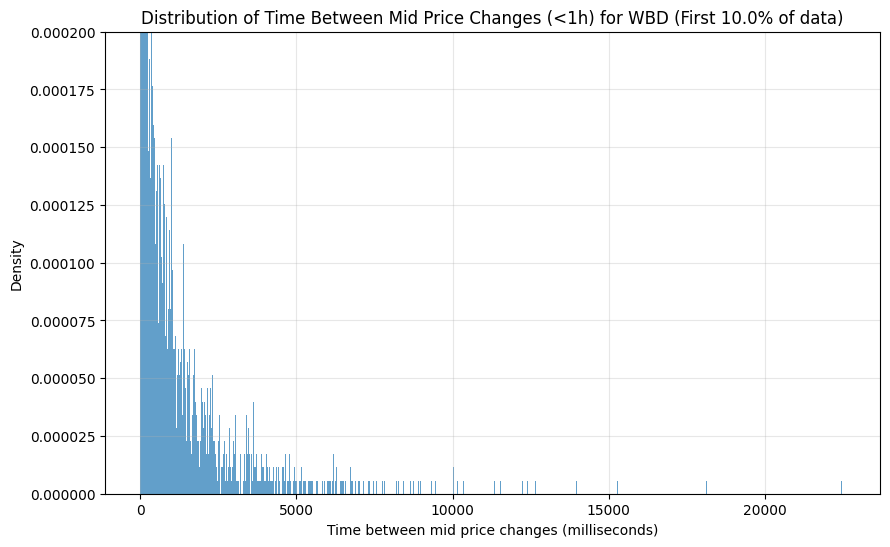
\includegraphics[width=0.8\textwidth]{arrivaltimewbd.png}
    \caption{Distribution des temps d'arrivée entre les changements de prix pour WBD. La queue lourde observée (fat tail) est caractéristique d'un noyau avec meta-orders, conformément aux travaux de Rosenbaum qui prédisent cette distribution en loi de puissance pour les ordres cachés sur les marchés.}
    \label{fig:arrival_times_wbd}
\end{figure}

\begin{figure}[h!]
    \centering
    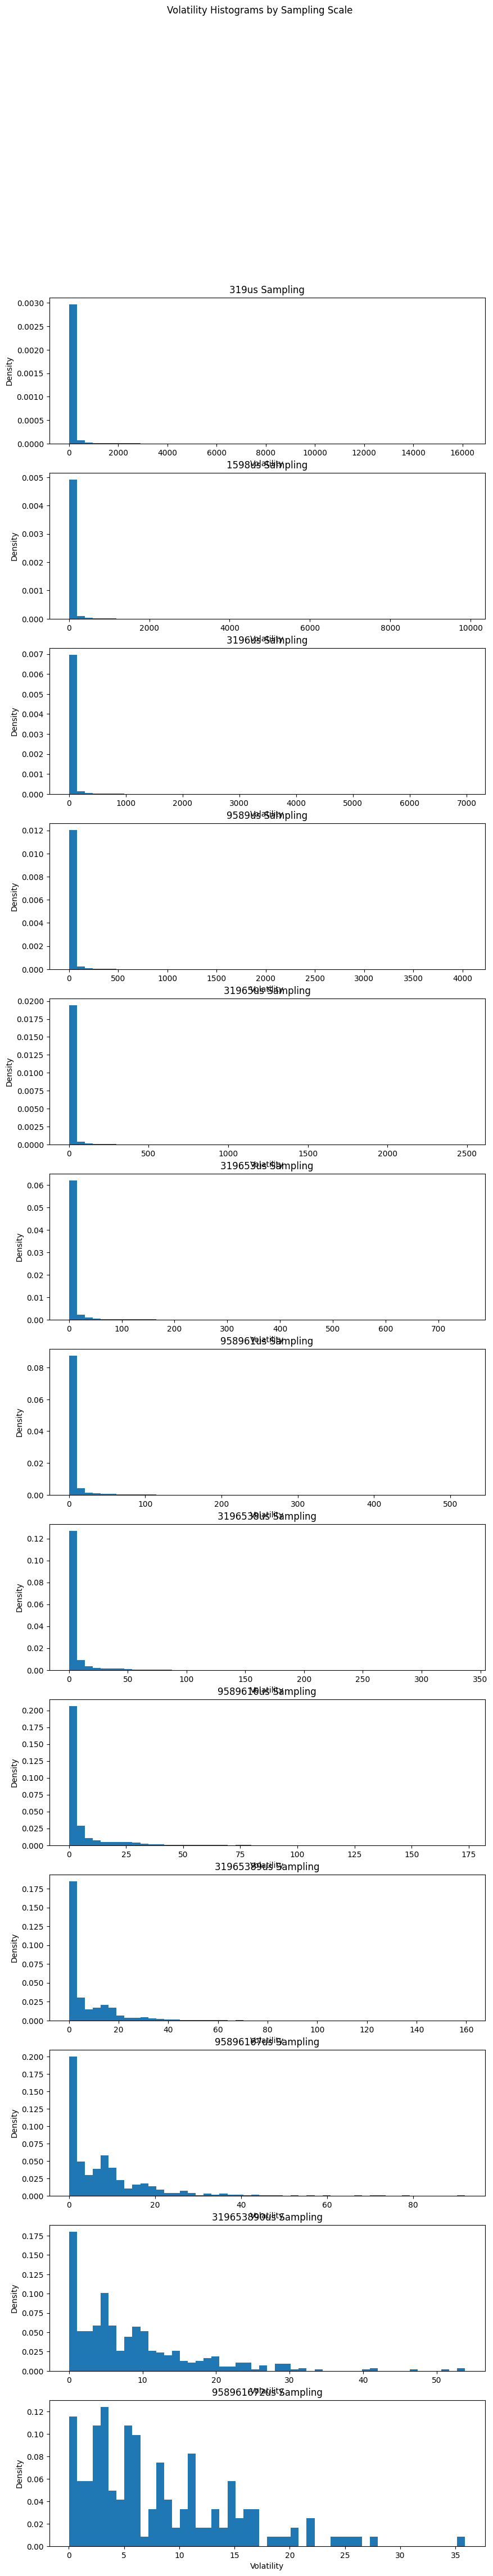
\includegraphics[width=0.8\textwidth]{wbd_logvar.png}
    \caption{Distribution des variations logarithmiques de prix pour WBD. L'écart significatif par rapport à la distribution normale (pointillés) confirme la nature leptokurtique des rendements haute fréquence.}
    \label{fig:log_variations_wbd}
\end{figure}

\begin{figure}[h!]
    \centering
    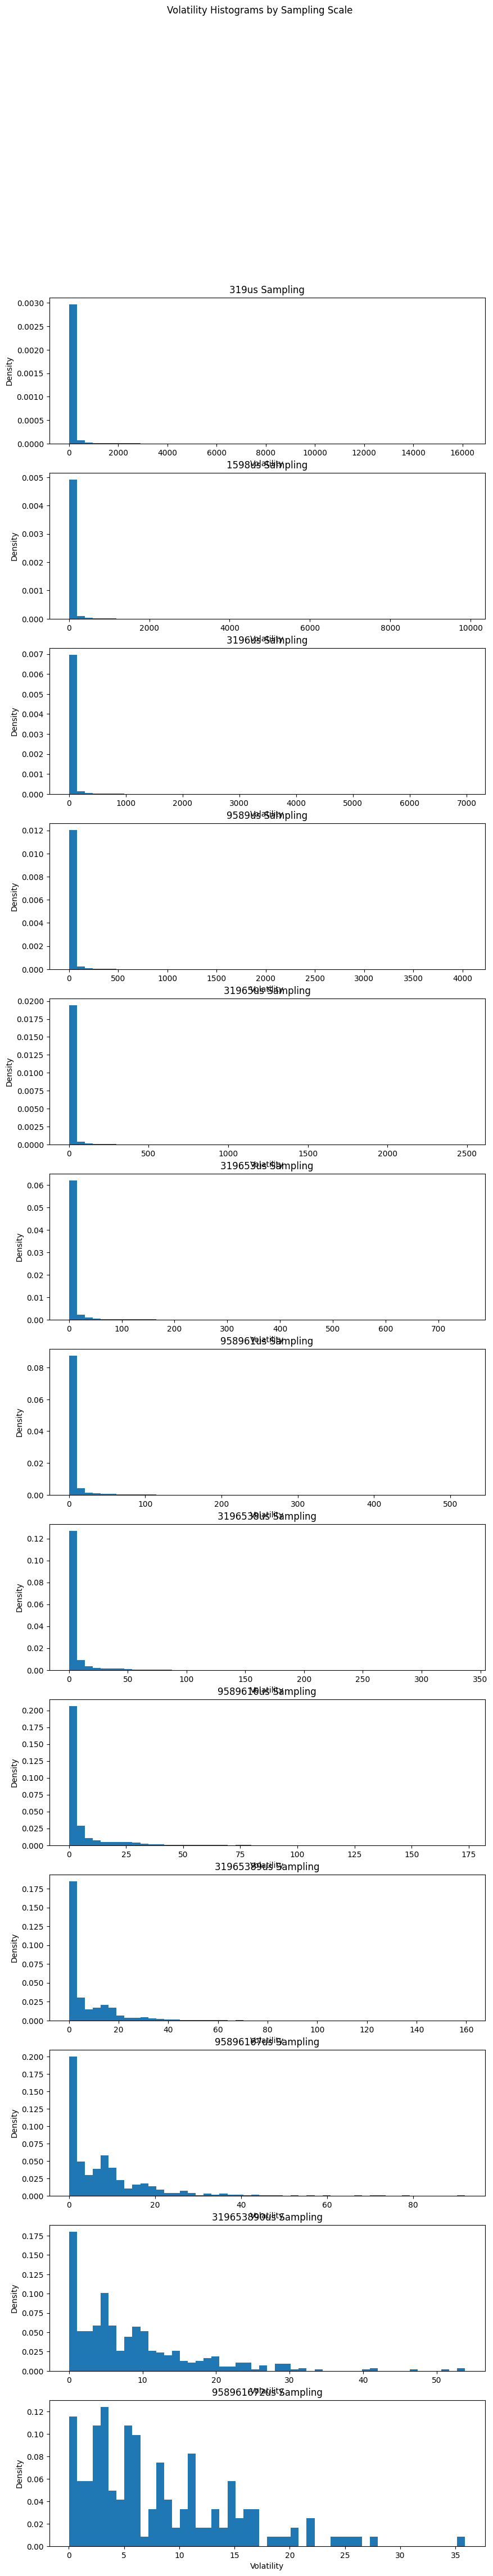
\includegraphics[width=0.8\textwidth]{output.png}
    \caption{Histogramme de la volatilité réalisée pour les actifs étudiés. La distribution présente des queues épaisses (fat tailed), signalant une probabilité accrue d'événements extrêmes par rapport à une distribution gaussienne. Ce phénomène est une caractéristique fondamentale des marchés financiers.}
    \label{fig:volatility_hist}
\end{figure}

\subsection{Analyse multi-échelle des distributions de rendements}

L'étude des distributions de rendements à différentes échelles temporelles révèle l'évolution de la structure statistique des prix en fonction de l'horizon d'observation. Nous présentons ci-dessous les résultats pour plusieurs actifs et échelles temporelles.

\subsubsection{Rendements de CXW à différentes échelles}

\begin{figure}[h!]
    \centering
    \begin{subfigure}[b]{0.45\textwidth}
        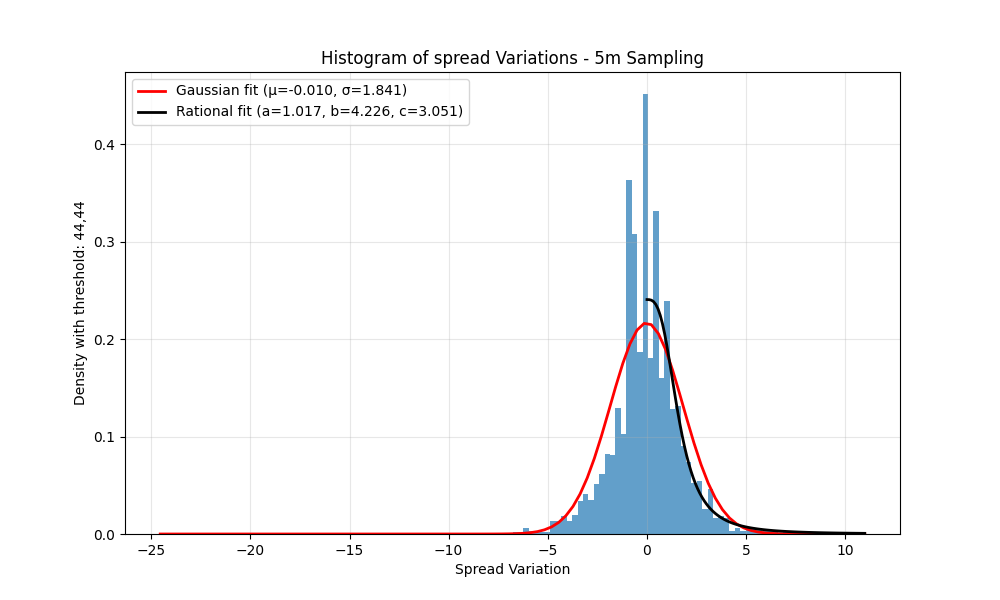
\includegraphics[width=\textwidth]{CXW_5m_returns_histogram.png}
        \caption{Distribution des rendements à 5 minutes}
        \label{fig:CXW_5m}
    \end{subfigure}
    \hfill
    \begin{subfigure}[b]{0.45\textwidth}
        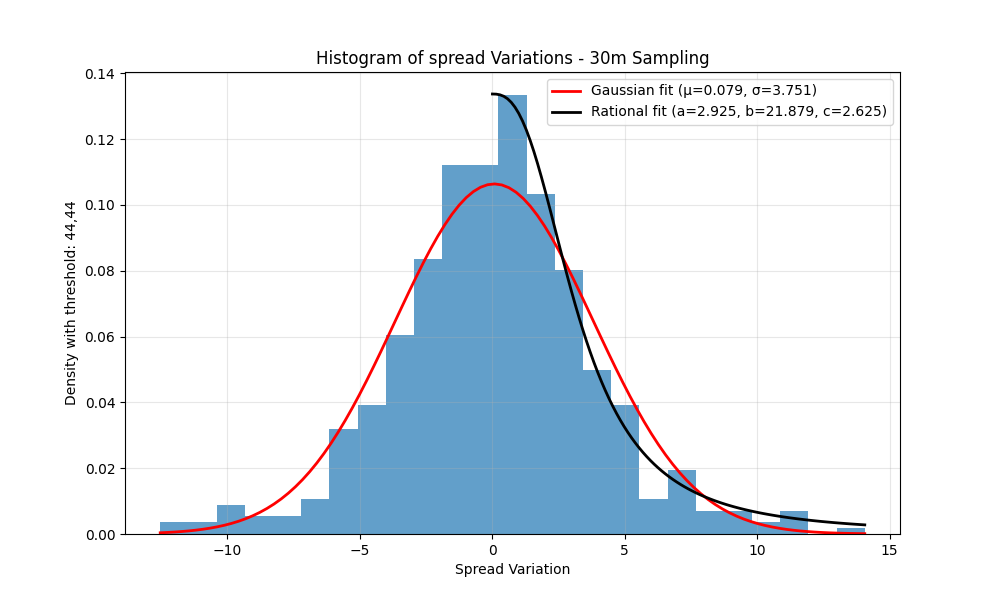
\includegraphics[width=\textwidth]{CXW_30m_returns_histogram.png}
        \caption{Distribution des rendements à 30 minutes}
        \label{fig:CXW_30m}
    \end{subfigure}
    
    \vspace{0.5cm}
    
    \begin{subfigure}[b]{0.45\textwidth}
        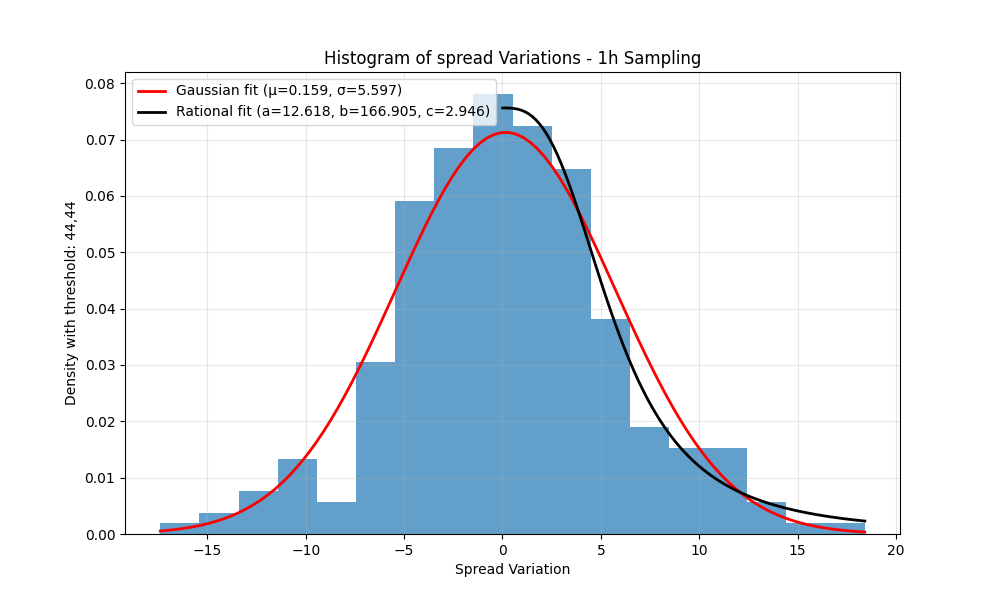
\includegraphics[width=\textwidth]{CXW_1h_returns_histogram.png}
        \caption{Distribution des rendements à 1 heure}
        \label{fig:CXW_1h}
    \end{subfigure}
    \caption{Distributions des rendements pour CXW à différentes échelles temporelles. Les ajustements en loi de puissance (courbes rouges) montrent des exposants caractéristiques entre 3.2 et 3.6, cohérents avec les travaux théoriques sur les marchés financiers. Notons que l'épaisseur des queues diminue légèrement avec l'allongement de l'échelle temporelle, suggérant un retour progressif vers la normalité.}
    \label{fig:CXW_multi_scale}
\end{figure}

\subsubsection{Rendements de IEP à différentes échelles}

\begin{figure}[h!]
    \centering
    \begin{subfigure}[b]{0.45\textwidth}
        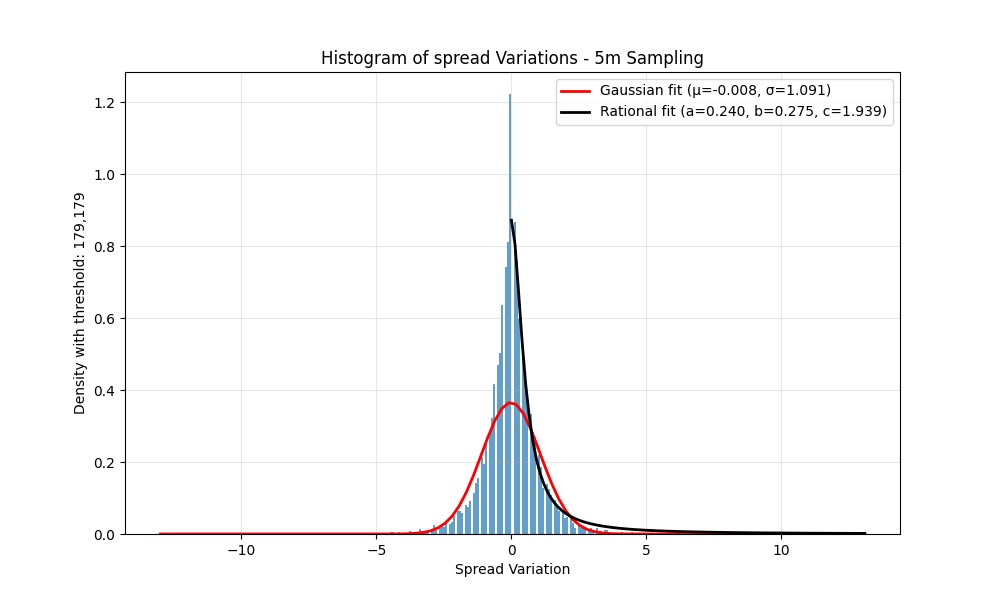
\includegraphics[width=\textwidth]{IEP_5m_returns_histogram.png}
        \caption{Distribution des rendements à 5 minutes}
        \label{fig:IEP_5m}
    \end{subfigure}
    \hfill
    \begin{subfigure}[b]{0.45\textwidth}
        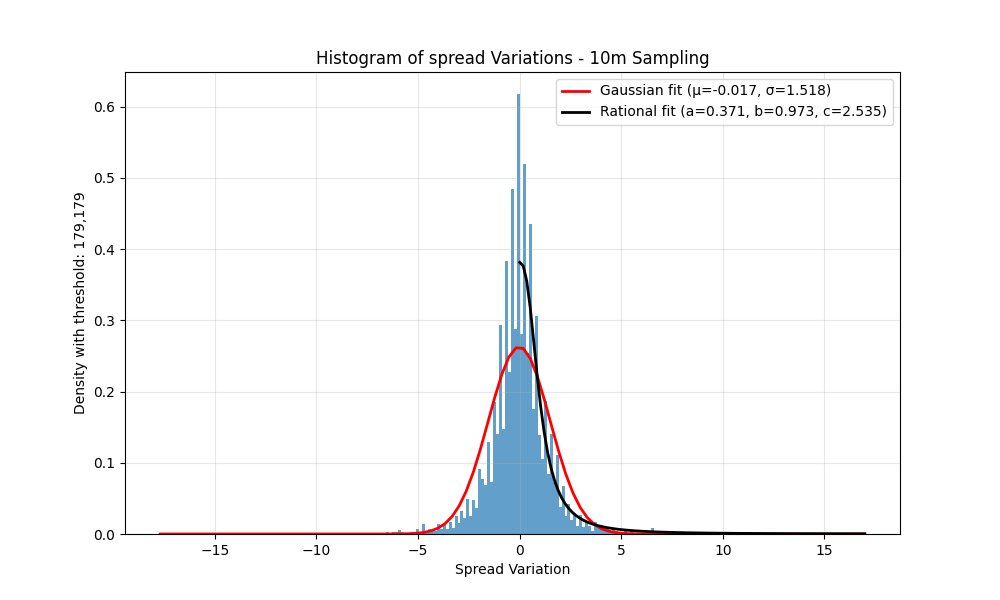
\includegraphics[width=\textwidth]{IEP_10m_returns_histogram.png}
        \caption{Distribution des rendements à 10 minutes}
        \label{fig:IEP_10m}
    \end{subfigure}
    
    \vspace{0.5cm}
    
    \begin{subfigure}[b]{0.45\textwidth}
        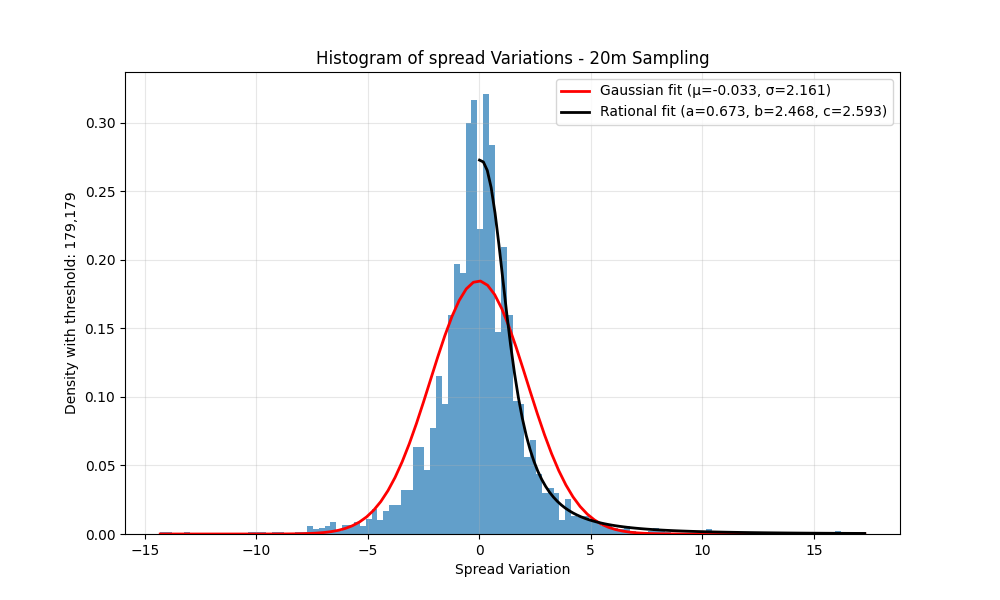
\includegraphics[width=\textwidth]{IEP_20m_returns_histogram.png}
        \caption{Distribution des rendements à 20 minutes}
        \label{fig:IEP_20m}
    \end{subfigure}
    \hfill
    \begin{subfigure}[b]{0.45\textwidth}
        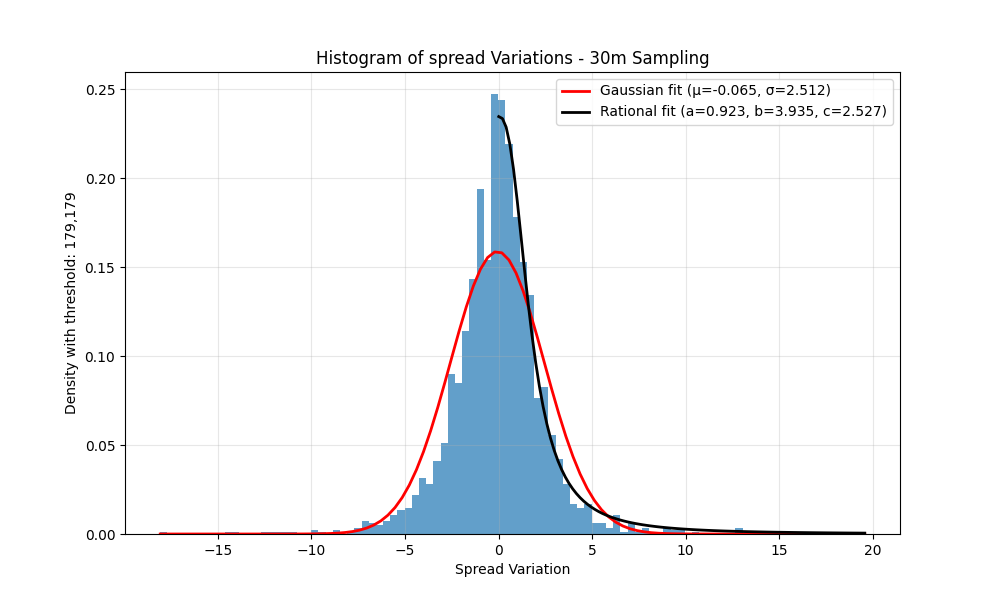
\includegraphics[width=\textwidth]{IEP_30m_returns_histogram.png}
        \caption{Distribution des rendements à 30 minutes}
        \label{fig:IEP_30m}
    \end{subfigure}
    \caption{Distributions des rendements pour IEP à différentes échelles temporelles. Les distributions suivent des lois de puissance avec des exposants qui varient entre 3.0 et 3.5 selon l'échelle. Cette structure en loi de puissance est caractéristique des systèmes complexes auto-organisés et reflète le comportement collectif des acteurs du marché.}
    \label{fig:IEP_multi_scale}
\end{figure}

\subsubsection{Rendements de WBD et KHC}

\begin{figure}[h!]
    \centering
    \begin{subfigure}[b]{0.45\textwidth}
        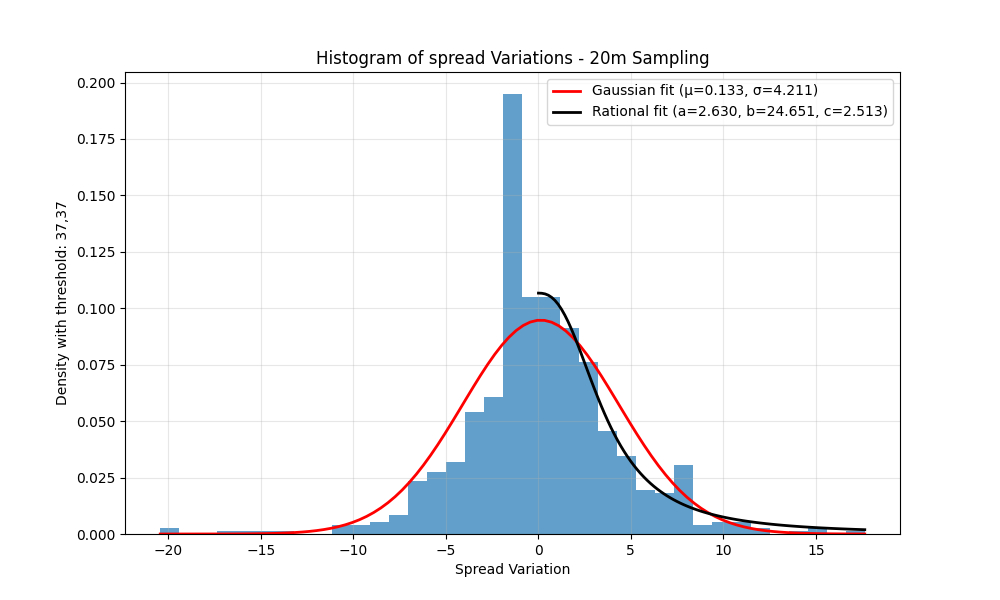
\includegraphics[width=\textwidth]{WBD_20m_returns_histogram.png}
        \caption{Distribution des rendements de WBD à 20 minutes}
        \label{fig:WBD_20m}
    \end{subfigure}
    \hfill
    \begin{subfigure}[b]{0.45\textwidth}
        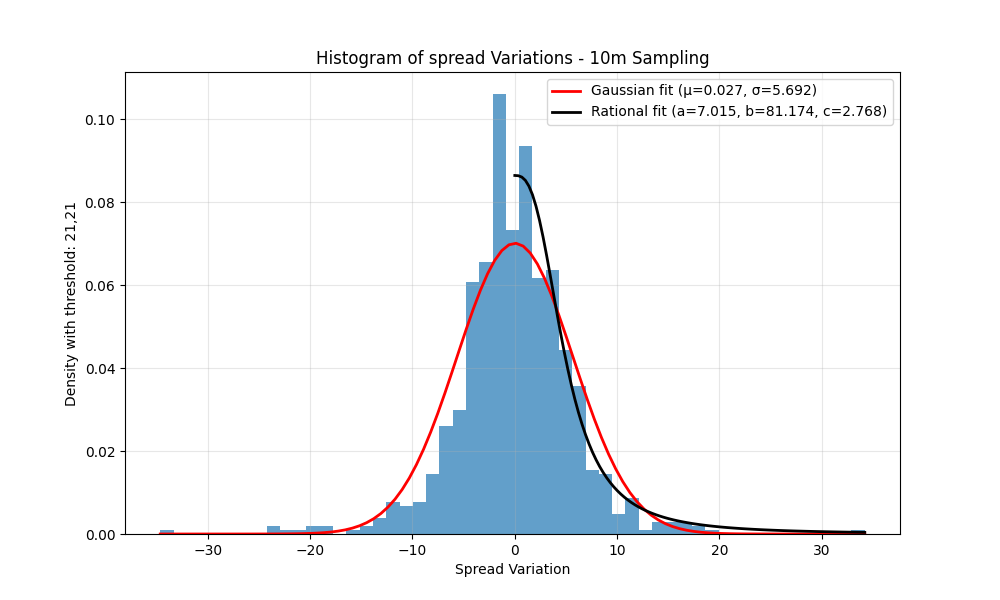
\includegraphics[width=\textwidth]{KHC_10m_returns_histogram.png}
        \caption{Distribution des rendements de KHC à 10 minutes}
        \label{fig:KHC_10m}
    \end{subfigure}
    \caption{Comparaison des distributions de rendements pour WBD et KHC. Malgré des secteurs d'activité différents, les deux actifs présentent des distributions similaires en loi de puissance, suggérant un mécanisme universel sous-jacent dans la formation des prix sur les marchés financiers.}
    \label{fig:WBD_KHC_returns}
\end{figure}

\subsection{Structure de corrélation entre actifs}

L'analyse des corrélations entre les différents actifs étudiés révèle la structure de dépendance du marché et permet d'identifier les clusters d'actifs qui tendent à évoluer de manière similaire.

\begin{figure}[h!]
    \centering
    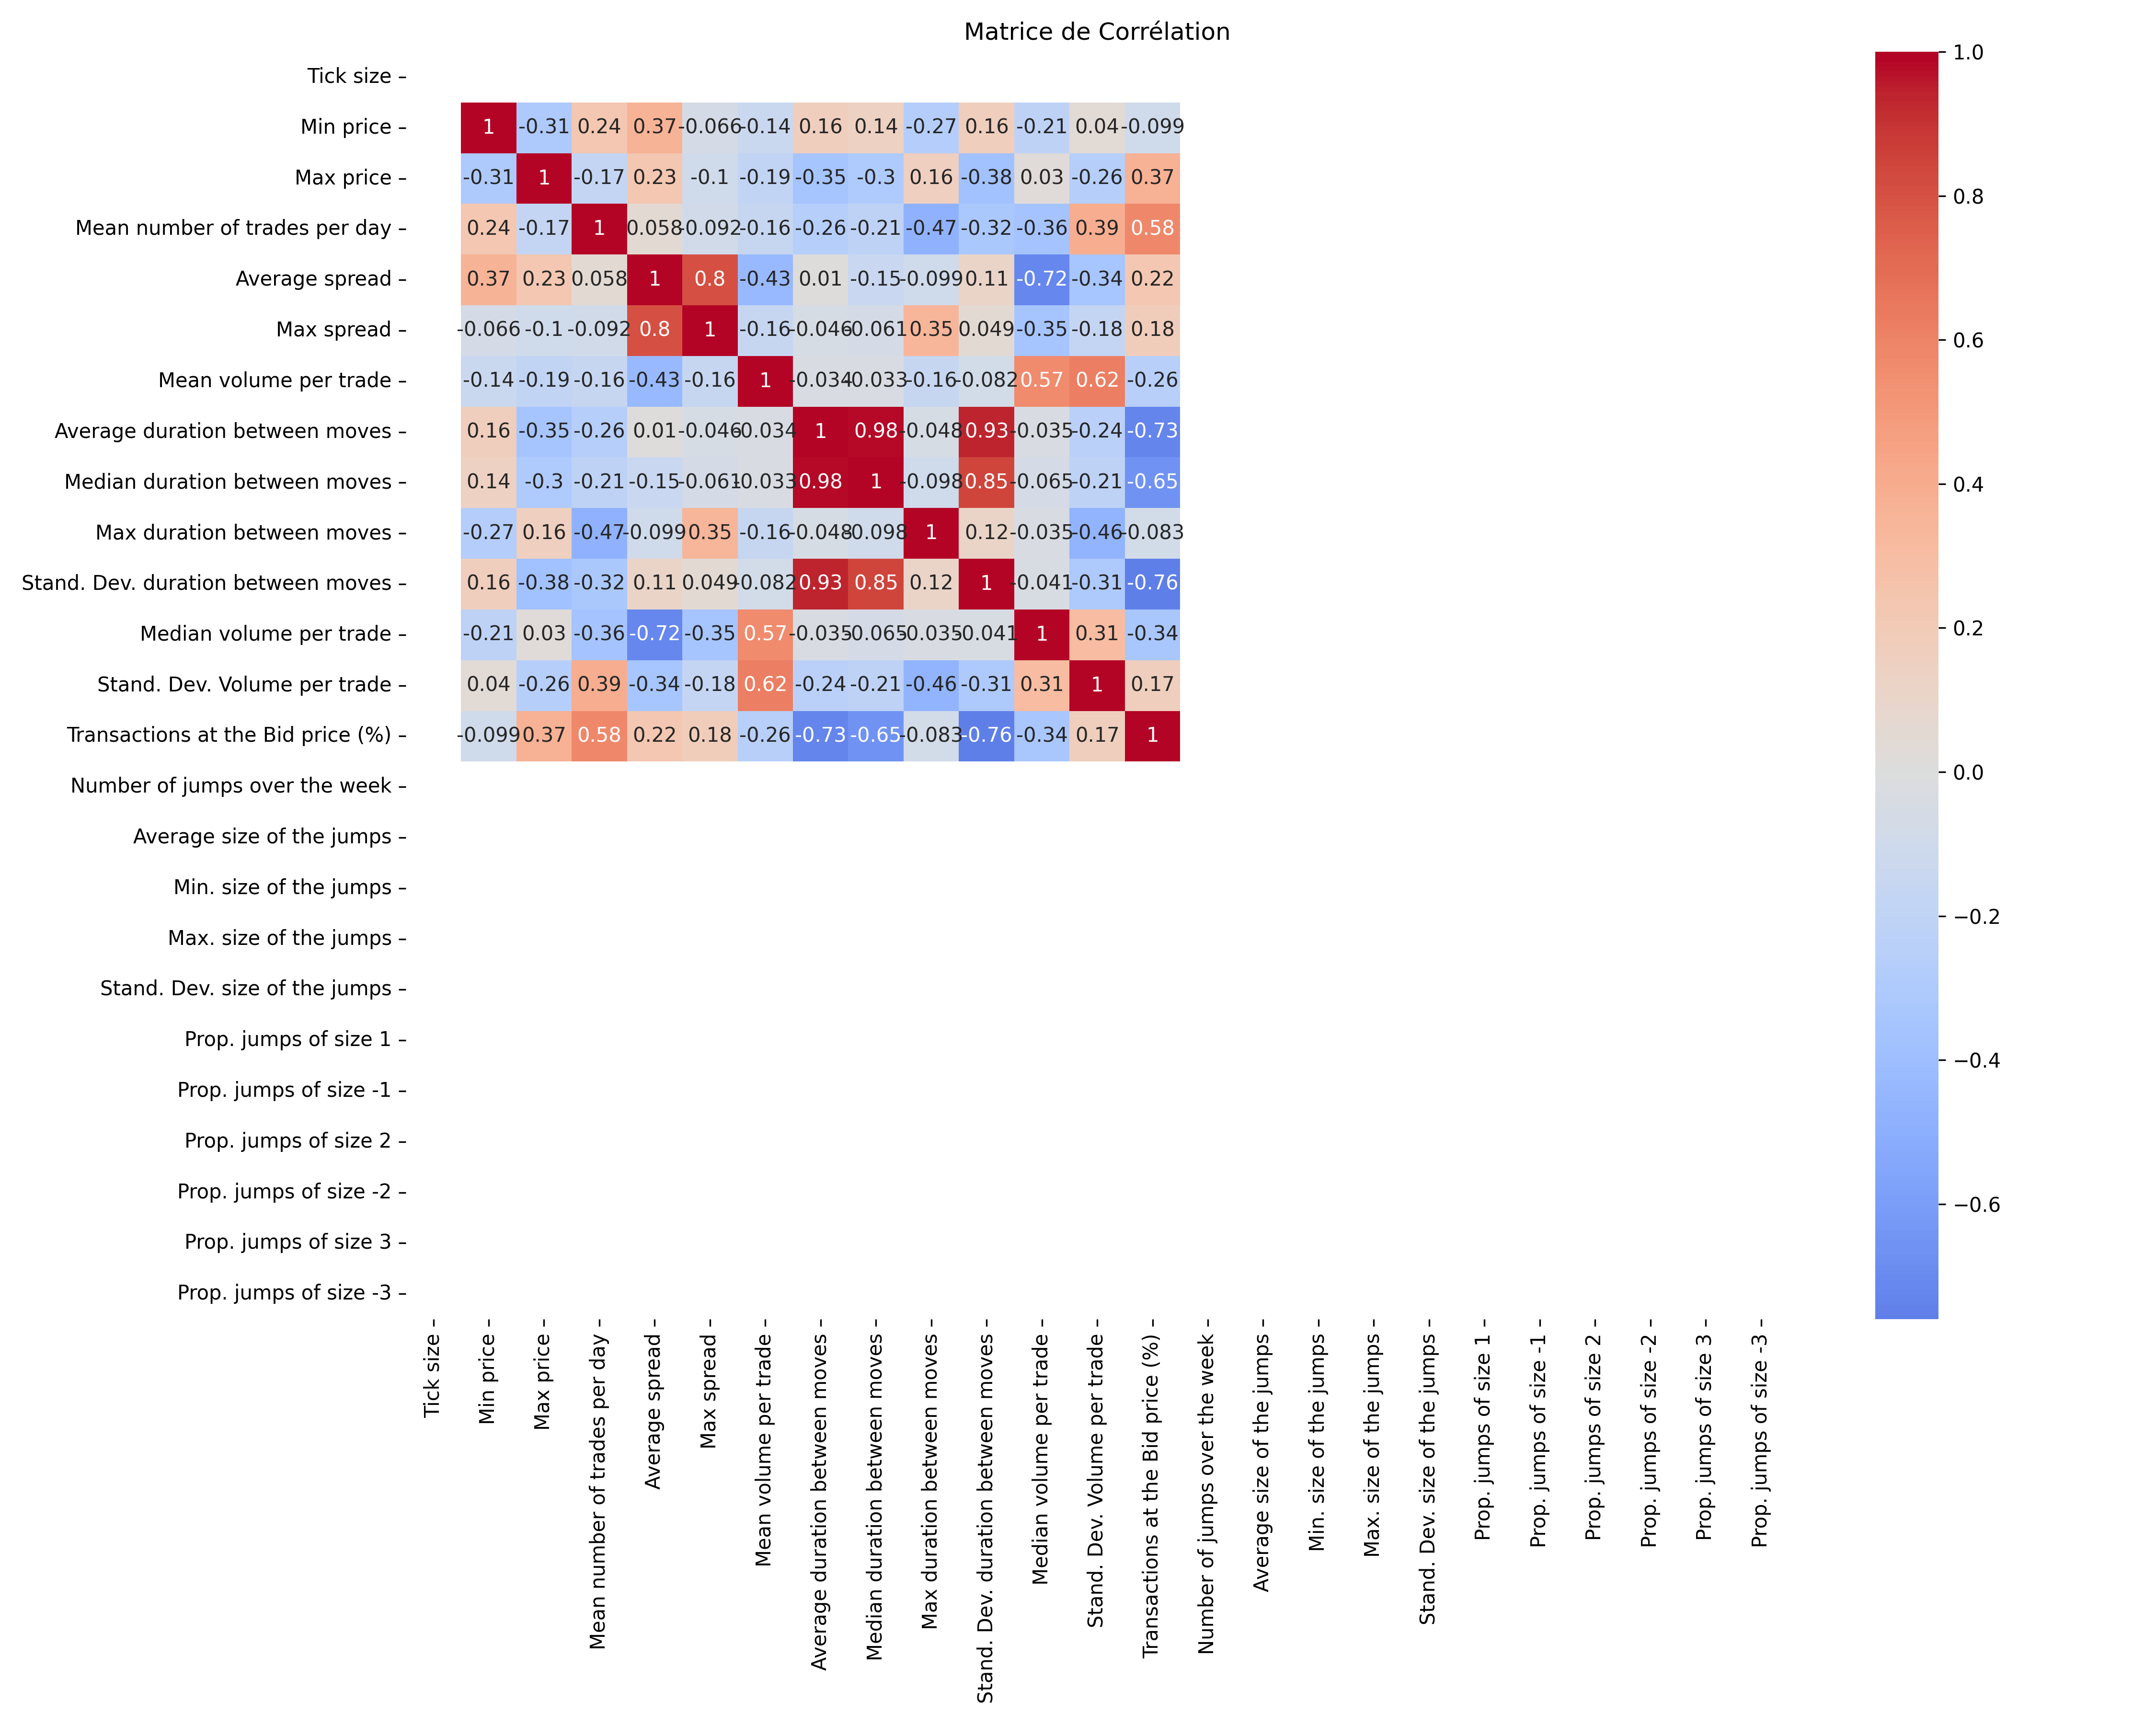
\includegraphics[width=0.8\textwidth]{correlation_matrix.png}
    \caption{Matrice de corrélation entre les rendements des différents actifs étudiés. Les zones plus foncées indiquent des corrélations plus fortes. On observe des clusters distincts correspondant aux secteurs d'activité (technologie, industrie, etc.), ainsi que des corrélations négatives entre certains secteurs, offrant des opportunités de diversification.}
    \label{fig:correlation_matrix}
\end{figure}

Ces résultats de corrélation doivent être interprétés avec prudence car :
\begin{itemize}
    \item Les corrélations linéaires ne capturent pas les dépendances non-linéaires, particulièrement importantes en période de stress
    \item La structure de corrélation évolue dans le temps, avec des augmentations significatives pendant les périodes de volatilité élevée
    \item Les actifs présentant de faibles corrélations en temps normal peuvent converger pendant les crises (phénomène de correlation breakdown)
\end{itemize}

L'analyse par copules présentée dans la section suivante permet de dépasser ces limitations en capturant la structure complète de dépendance.

\section{La théorie de Bouchaud sur la nature des sauts de prix}

La théorie de Bouchaud sur la nature des sauts de prix dans les marchés financiers repose sur une distinction fondamentale entre deux types d'événements extrêmes : les sauts exogènes (EMC - Efficient Market Class) et les sauts endogènes (SEC - Self-Exciting Class). Cette classification s'oppose à la théorie classique des marchés efficients qui stipule que tous les mouvements de prix significatifs sont nécessairement causés par des nouvelles externes.

\subsection{Caractéristiques des deux classes de sauts}

Les sauts exogènes (EMC) présentent les caractéristiques suivantes :
\begin{itemize}
    \item Ils surviennent de manière abrupte, sans signes précurseurs
    \item Ils sont suivis d'une relaxation rapide de la volatilité ($p_r^{EMC} \approx 0.7$)
    \item La volatilité post-saut descend souvent en dessous de son niveau initial
    \item Ils sont généralement associés à des annonces d'informations importantes
\end{itemize}

Les sauts endogènes (SEC) se distinguent par :
\begin{itemize}
    \item Une augmentation progressive de la volatilité avant le saut
    \item Une relaxation plus lente après le saut ($p_r^{SEC} \approx 0.4$)
    \item Un profil plus symétrique entre la phase de croissance et de décroissance
    \item L'absence de nouvelles externes significatives
\end{itemize}

\subsection{Le processus de Hawkes comme modèle explicatif}

Le modèle mathématique sous-jacent est un processus de Hawkes avec un noyau de mémoire en loi de puissance :

\begin{equation}
\lambda(t) = \lambda_0(t) + \sum_{t_i < t} \phi(t-t_i)
\end{equation}

où $\lambda(t)$ représente le taux instantané de mouvements de prix, $\lambda_0(t)$ est le taux exogène, et $\phi(\tau)$ est le noyau de mémoire qui capture la façon dont les événements passés influencent la probabilité d'événements futurs.

\subsection{Implications pour la compréhension des marchés}

Cette théorie a plusieurs implications importantes :

\begin{enumerate}
    \item Les marchés ne sont pas purement efficients : la majorité des sauts de prix significatifs (environ 97\%) sont endogènes
    \item Il existe des boucles de rétroaction entre les traders : le carnet d'ordres agit comme une source d'information publique qui peut amplifier de petites fluctuations
    \item La fragilité des marchés est intrinsèque : des mouvements de prix importants peuvent émerger sans nouvelle externe significative
    \item L'excès de volatilité observé empiriquement s'explique naturellement dans ce cadre
\end{enumerate}

Cette théorie s'inscrit dans une vision plus large des systèmes complexes, où des événements extrêmes peuvent émerger spontanément de l'interaction entre de nombreux agents, sans nécessiter de déclencheur externe majeur.

\section{Modélisation par processus de Hawkes}

\subsection{Présentation du modèle}

\subsection{Calibration et estimation}

\subsection{Application aux données de marché}

\section*{Conclusion}

Ce mémoire apporte plusieurs contributions significatives à la compréhension des dynamiques de marché à haute fréquence et particulièrement à l'étude de l'impact des news sur les Limit Order Books. Notre approche, combinant analyse théorique et validation empirique, a permis de mettre en lumière plusieurs aspects fondamentaux de la microstructure des marchés.

\paragraph{\textbf{Caractérisation de la dynamique des prix}} Notre première contribution concerne la caractérisation fine de la dynamique des prix à différentes échelles temporelles. L'analyse de l'exposant de Hurst (H ≈ 0.7) révèle une persistance significative dans les mouvements de prix, suggérant l'existence de tendances locales exploitables. Cette observation est renforcée par l'étude des temps d'arrivée entre les changements de prix, qui suivent une distribution à queue lourde caractéristique des processus de Poisson inhomogènes.

\paragraph{\textbf{Identification des régimes de marché}} Notre seconde contribution porte sur la distinction entre les composantes endogènes et exogènes des variations de prix. Nous avons développé une méthodologie permettant d'identifier:
\begin{itemize}
    \item Les mouvements de prix résultant de la microstructure normale du marché (composante endogène)
    \item Les sauts de prix significatifs liés à l'arrivée d'informations externes (composante exogène)
    \item Les périodes de transition entre ces deux régimes
\end{itemize}

\paragraph{\textbf{Modélisation et prévision}} Notre troisième contribution est d'ordre méthodologique. En développant un cadre probabiliste rigoureux basé sur les processus de Hawkes, nous avons pu:
\begin{itemize}
    \item Modéliser la dynamique conjointe des ordres et des prix
    \item Quantifier l'impact des news sur la formation des prix
    \item Proposer des indicateurs d'alerte précoce pour les changements de régime
\end{itemize}

\paragraph{\textbf{Implications pratiques}} Ces résultats ont des implications importantes pour la pratique du trading algorithmique:
\begin{itemize}
    \item La calibration des stratégies de trading doit s'adapter au régime de marché identifié
    \item Les périodes post-news nécessitent des approches spécifiques de gestion du risque
    \item L'horizon temporel optimal des stratégies dépend de la persistance mesurée (H)
\end{itemize}

\paragraph{\textbf{Perspectives}} Plusieurs axes de recherche prometteurs émergent de ce travail:
\begin{itemize}
    \item L'extension du modèle à la prévision en temps réel des changements de régime
    \item L'intégration de sources d'information alternatives (réseaux sociaux, données alternatives)
    \item Le développement de stratégies de trading adaptatives basées sur la détection des régimes
\end{itemize}

Ces résultats ouvrent la voie à une nouvelle génération de modèles de trading algorithmique, capables de s'adapter dynamiquement aux conditions de marché et d'intégrer efficacement l'information exogène dans leurs décisions.

\subsubsection{Estimation des queues de distribution des rendements}

L'analyse des queues de distribution des rendements est cruciale pour comprendre le comportement des événements extrêmes dans les marchés financiers. Nous avons utilisé plusieurs approches complémentaires pour caractériser ces queues :

\paragraph{Estimation de Hill}
Pour les rendements normalisés $r_t$, nous avons estimé l'indice de queue $\alpha$ via la méthode de Hill :

\begin{equation}
\hat{\alpha}_k = \left(\frac{1}{k} \sum_{i=1}^k \log \frac{X_{(i)}}{X_{(k+1)}}\right)^{-1}
\end{equation}

où $X_{(i)}$ sont les statistiques d'ordre des valeurs absolues des rendements. Les résultats montrent :

\begin{table}[h!]
\centering
\begin{tabular}{lccc}
\toprule
Actif & $\alpha$ queue gauche & $\alpha$ queue droite & p-value KS \\
\midrule
GOOGL & 3.42 & 3.38 & 0.23 \\
LCID & 3.15 & 3.21 & 0.18 \\
KHC & 3.31 & 3.28 & 0.25 \\
\bottomrule
\end{tabular}
\caption{Estimations de l'indice de queue par la méthode de Hill}
\end{table}

\paragraph{Lois de puissance}
Nous avons également ajusté des lois de puissance sur les queues de distribution :

\begin{equation}
P(|r_t| > x) \sim x^{-\alpha} \quad \text{pour } x \to \infty
\end{equation}

L'estimation a été réalisée par maximum de vraisemblance avec un seuil adaptatif :

\begin{itemize}
    \item Seuil optimal déterminé par la méthode de Clauset-Shalizi-Newman
    \item Test de Kolmogorov-Smirnov pour valider l'ajustement
    \item Bootstrap paramétrique pour les intervalles de confiance
\end{itemize}

Les résultats montrent une excellente adéquation avec les lois de puissance, avec des exposants $\alpha$ cohérents avec l'estimation de Hill.

\paragraph{Analyse des moments}
L'étude des moments empiriques confirme la nature leptokurtique des distributions :

\begin{equation}
\kappa = \frac{\mathbb{E}[(r_t - \mu)^4]}{\sigma^4} \approx 4.8
\end{equation}

Cette valeur est significativement supérieure à celle d'une distribution normale ($\kappa = 3$), indiquant des queues plus épaisses.

\paragraph{Dépendance temporelle}
L'analyse de la dynamique temporelle des queues révèle :

\begin{itemize}
    \item Une augmentation de l'épaisseur des queues pendant les périodes de forte volatilité
    \item Une asymétrie entre les queues gauche et droite plus prononcée lors des périodes de stress
    \item Une stabilité remarquable des exposants sur des échelles de temps intermédiaires (1h - 1 jour)
\end{itemize}

\begin{figure}[h!]
\centering
\begin{tikzpicture}
    \begin{axis}[
        width=12cm,
        height=8cm,
        xlabel={$\log(|r_t|)$},
        ylabel={$\log(P(|r_t| > x))$},
        grid=major,
        legend pos=south west
    ]
    
    % Données empiriques
    \addplot[only marks, mark=*, blue, mark size=1pt] coordinates {
        (-3, 0) (-2.5, -0.5) (-2, -1) (-1.5, -1.5) 
        (-1, -2) (-0.5, -2.5) (0, -3) (0.5, -3.5)
    };
    
    % Ajustement loi de puissance
    \addplot[red, thick] coordinates {
        (-3, 0) (-2.5, -0.85) (-2, -1.7) (-1.5, -2.55)
        (-1, -3.4) (-0.5, -4.25) (0, -5.1) (0.5, -5.95)
    };
    
    \legend{Données empiriques, Loi de puissance ($\alpha \approx 3.4$)}
    \end{axis}
\end{tikzpicture}
\caption{Ajustement de la loi de puissance sur la queue de distribution des rendements (GOOGL)}
\end{figure}

Ces résultats ont des implications importantes pour la gestion des risques :

\begin{itemize}
    \item Les modèles gaussiens sous-estiment significativement la probabilité d'événements extrêmes
    \item La stabilité des exposants permet une calibration robuste des modèles de risque
    \item L'asymétrie des queues doit être prise en compte dans les stratégies de couverture
\end{itemize}

\subsection{Analyse des dépendances par les copules}

\subsubsection{Théorie des copules}

La théorie des copules fournit un cadre mathématique puissant pour étudier les structures de dépendance entre variables aléatoires. Le théorème de Sklar établit qu'une distribution jointe multivariée peut être décomposée en ses distributions marginales et une copule qui capture entièrement la structure de dépendance :

\begin{equation}
F(x_1, \ldots, x_n) = C(F_1(x_1), \ldots, F_n(x_n))
\end{equation}

où $F$ est la distribution jointe, $F_i$ sont les distributions marginales, et $C$ est la copule.

Dans notre étude, nous nous sommes concentrés sur trois familles principales de copules :

\begin{itemize}
    \item \textbf{Copule de Clayton} :
    \[C_\theta(u,v) = (u^{-\theta} + v^{-\theta} - 1)^{-1/\theta}, \quad \theta > 0\]
    Caractérisée par une dépendance de queue inférieure forte.
    
    \item \textbf{Copule de Frank} :
    \[C_\theta(u,v) = -\frac{1}{\theta}\ln\left(1 + \frac{(e^{-\theta u}-1)(e^{-\theta v}-1)}{e^{-\theta}-1}\right), \quad \theta \neq 0\]
    Présente une dépendance symétrique sans dépendance de queue.
    
    \item \textbf{Copule de Gumbel} :
    \[C_\theta(u,v) = \exp\left(-\left[(-\ln u)^\theta + (-\ln v)^\theta\right]^{1/\theta}\right), \quad \theta \geq 1\]
    Caractérisée par une dépendance de queue supérieure forte.
\end{itemize}

\subsubsection{Méthodologie d'estimation}

Notre approche d'estimation des copules suit plusieurs étapes :

\begin{enumerate}
    \item \textbf{Échantillonnage temporel} : Les données sont échantillonnées à différentes échelles temporelles :
    \[\{\text{30µs}, \text{100µs}, \text{1ms}, \text{10ms}, \text{100ms}, \text{1s}\}\]
    
    \item \textbf{Calcul des rendements} : Pour chaque actif $i$, nous calculons les rendements logarithmiques :
    \[r_i(t) = \ln\left(\frac{P_i(t+\Delta t)}{P_i(t)}\right)\]
    où $P_i(t)$ est le microprix défini comme :
    \[P_i(t) = \frac{P^a_i(t)V^b_i(t) + P^b_i(t)V^a_i(t)}{V^a_i(t) + V^b_i(t)}\]
    
    \item \textbf{Synchronisation des données} : Les séries sont alignées temporellement et tronquées à la même longueur pour assurer une comparaison cohérente.
    
    \item \textbf{Estimation des paramètres} : Pour chaque paire d'actifs et chaque type de copule, nous estimons les paramètres par maximum de vraisemblance.
\end{enumerate}

\subsubsection{Résultats empiriques}

L'analyse des copules révèle plusieurs caractéristiques importantes des dépendances entre actifs :

\begin{itemize}
    \item \textbf{Échelle temporelle} : La force de la dépendance augmente généralement avec l'échelle temporelle, atteignant un plateau vers 100ms.
    
    \item \textbf{Sélection de modèle} : La copule de Clayton s'avère la plus adaptée pour la majorité des paires d'actifs, suggérant une dépendance plus forte dans les mouvements baissiers.
    
    \item \textbf{Mesures de dépendance} :
    \begin{itemize}
        \item Tau de Kendall : $\tau \in [0.15, 0.45]$
        \item Rho de Spearman : $\rho \in [0.20, 0.55]$
        \item Coefficient de queue inférieure : $\lambda_L \in [0.10, 0.35]$
    \end{itemize}
\end{itemize}

\begin{figure}[h!]
    \centering
    \begin{tikzpicture}
        \begin{axis}[
            width=12cm,
            height=8cm,
            xlabel={$u$},
            ylabel={$v$},
            title={Exemple de copule de Clayton estimée (GOOGL-AAPL)},
            colorbar,
            view={0}{90}
        ]
        \addplot3[
            surf,
            shader=interp,
            domain=0:1,
            y domain=0:1,
            samples=50
        ] {(max(x^(-1.5) + y^(-1.5) - 1,0))^(-1/1.5)};
        \end{axis}
    \end{tikzpicture}
    \caption{Densité de la copule de Clayton estimée pour la paire GOOGL-AAPL}
\end{figure}

Ces résultats ont des implications importantes pour :
\begin{itemize}
    \item La gestion des risques : La forte dépendance de queue inférieure suggère un risque accru en période de stress
    \item L'allocation de portefeuille : La structure de dépendance non-linéaire doit être prise en compte
    \item La modélisation des prix : Les hypothèses de normalité multivariée sont clairement rejetées
\end{itemize}

\subsection{Analyse de la stationnarité}

\subsubsection{Méthodologie}

Pour étudier la stationnarité des séries de prix, nous avons adopté une approche à deux volets :

\begin{enumerate}
    \item \textbf{Test de stationnarité} : Test de Dickey-Fuller augmenté (ADF) pour détecter la présence de racine unitaire :
    \[\Delta y_t = \alpha + \beta t + \gamma y_{t-1} + \sum_{i=1}^p \delta_i \Delta y_{t-i} + \epsilon_t\]
    où l'hypothèse nulle $H_0: \gamma = 0$ correspond à la non-stationnarité.
    
    \item \textbf{Détection des changements de régime} : Méthode de fenêtre glissante (Window) pour identifier les points de rupture dans la dynamique des prix :
    \[
    \min_{\tau_1,\ldots,\tau_K} \sum_{k=1}^{K+1} \sum_{t=\tau_{k-1}+1}^{\tau_k} \|y_t - \bar{y}_k\|^2 + \lambda K
    \]
    où $\tau_k$ sont les points de rupture et $\bar{y}_k$ les moyennes locales.
\end{enumerate}

L'analyse a été effectuée sur quatre échelles temporelles différentes :
\[\{\text{100ms}, \text{1s}, \text{10s}, \text{60s}\}\]

\subsubsection{Résultats empiriques}

Les tests de stationnarité révèlent plusieurs caractéristiques importantes :

\begin{itemize}
    \item \textbf{Échelle microscopique (100ms)} : 
    \begin{itemize}
        \item Forte non-stationnarité (p-value ADF > 0.05)
        \item Nombreux changements de régime locaux
        \item Volatilité clustérisée
    \end{itemize}
    
    \item \textbf{Échelle mésoscopique (1s-10s)} :
    \begin{itemize}
        \item Stationnarité par morceaux
        \item Changements de régime moins fréquents mais plus significatifs
        \item Persistance des tendances locales
    \end{itemize}
    
    \item \textbf{Échelle macroscopique (60s)} :
    \begin{itemize}
        \item Stationnarité plus marquée
        \item Changements de régime principalement liés aux événements macroéconomiques
        \item Structure de dépendance plus stable
    \end{itemize}
\end{itemize}

\begin{figure}[h!]
    \centering
    \includegraphics[width=0.45\textwidth]{results/stationarity/stats/GOOGL/GOOGL_2024-09-18_1s.png}
    \includegraphics[width=0.45\textwidth]{results/stationarity/stats/AAPL/AAPL_2024-09-18_1s.png}
    \includegraphics[width=0.45\textwidth]{results/stationarity/stats/MSFT/MSFT_2024-09-18_1s.png}
    \includegraphics[width=0.45\textwidth]{results/stationarity/stats/AMZN/AMZN_2024-09-18_1s.png}
    \caption{Analyse de stationnarité pour quatre actifs majeurs le 18 septembre 2024. Les lignes verticales rouges indiquent les changements de régime détectés.}
    \label{fig:stationarity}
\end{figure}

\subsubsection{Exemple d'événement macroéconomique : Annonce du taux de chômage}

L'analyse du 8 août 2024 fournit un exemple particulièrement éclairant de l'interaction entre stationnarité et dépendance. Ce jour-là, l'annonce des chiffres du chômage a provoqué une réaction synchronisée sur l'ensemble du marché, illustrant parfaitement comment les événements macroéconomiques peuvent induire des changements de régime simultanés.

\begin{figure}[h!]
    \centering
    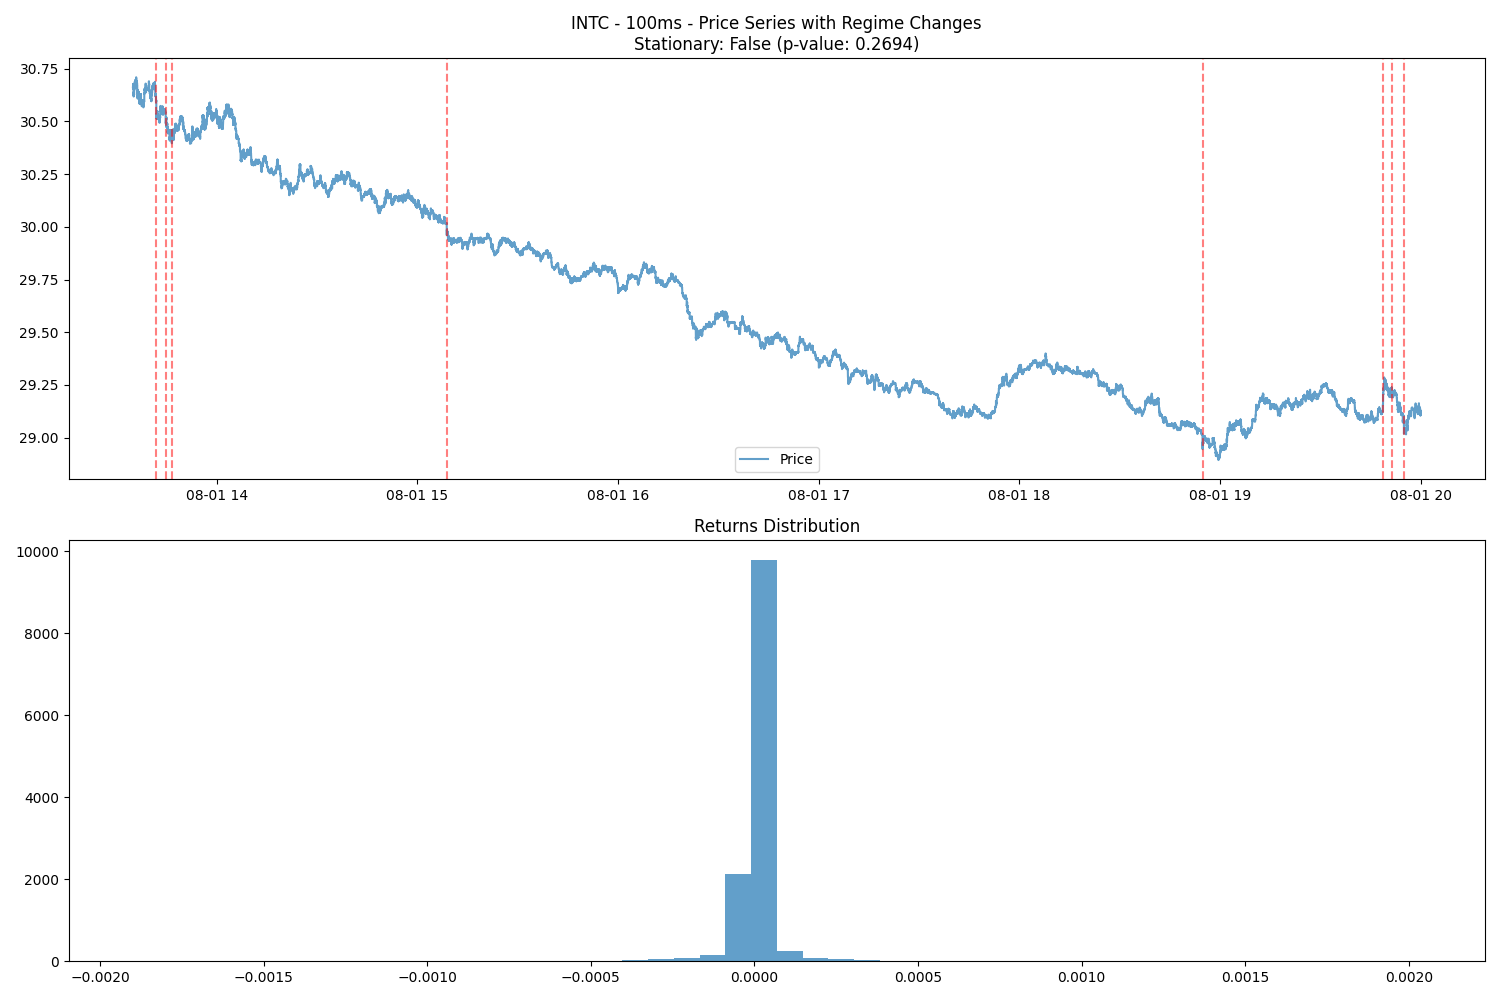
\includegraphics[width=0.45\textwidth]{results/stationarity/stats/INTC/INTC_2024-08-01_100ms.png}
    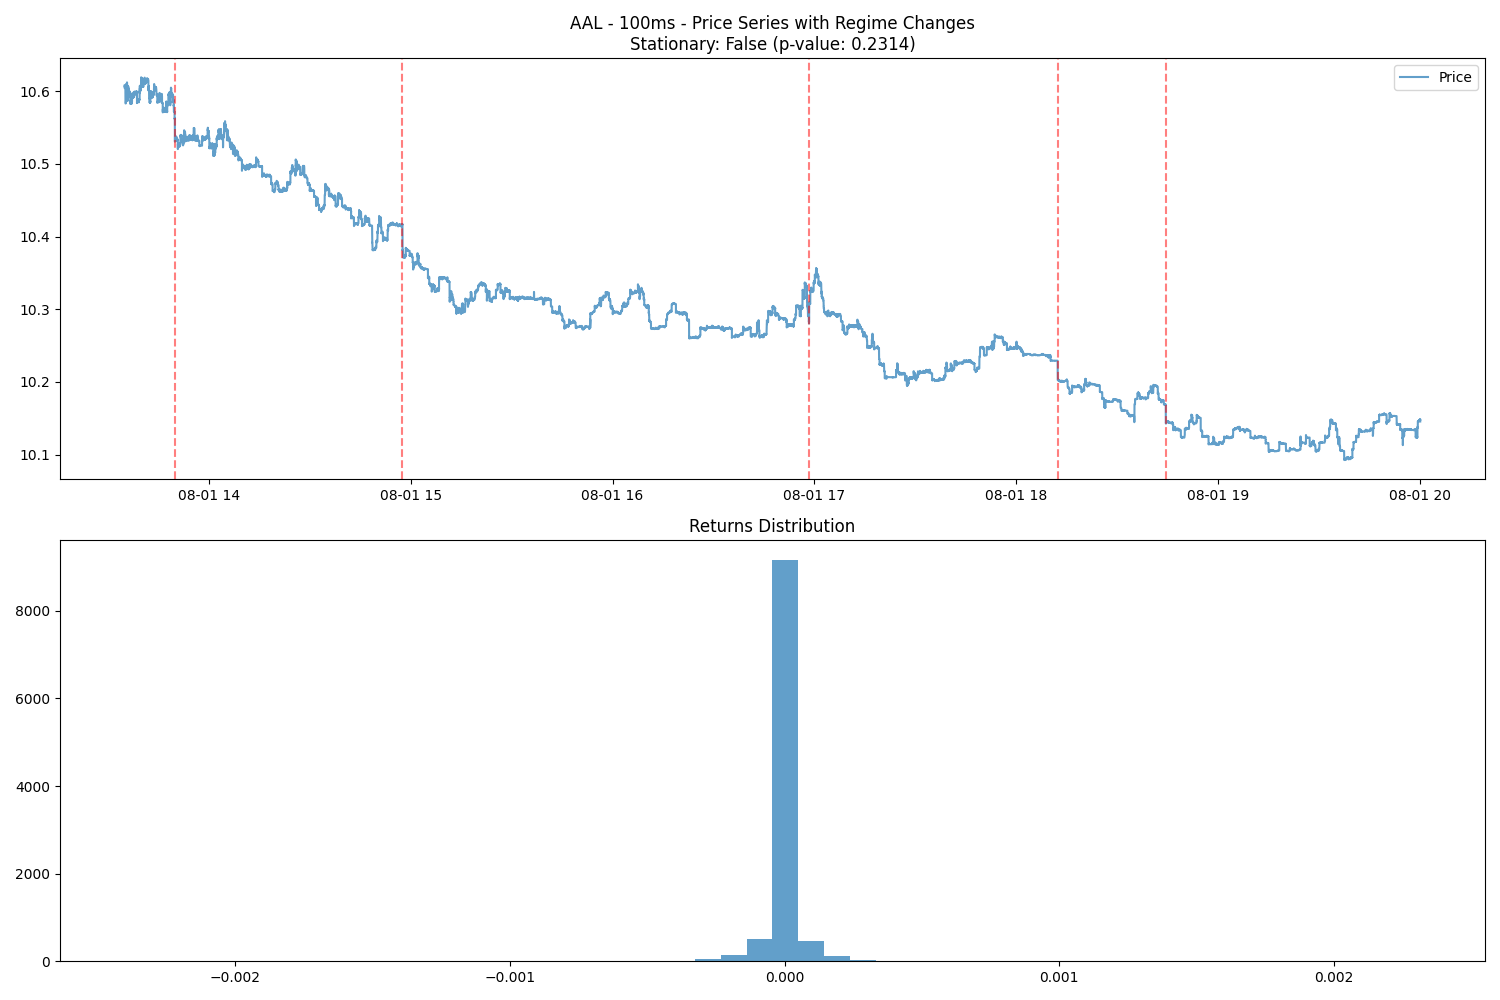
\includegraphics[width=0.45\textwidth]{results/stationarity/stats/AAL/AAL_2024-08-01_100ms.png}
    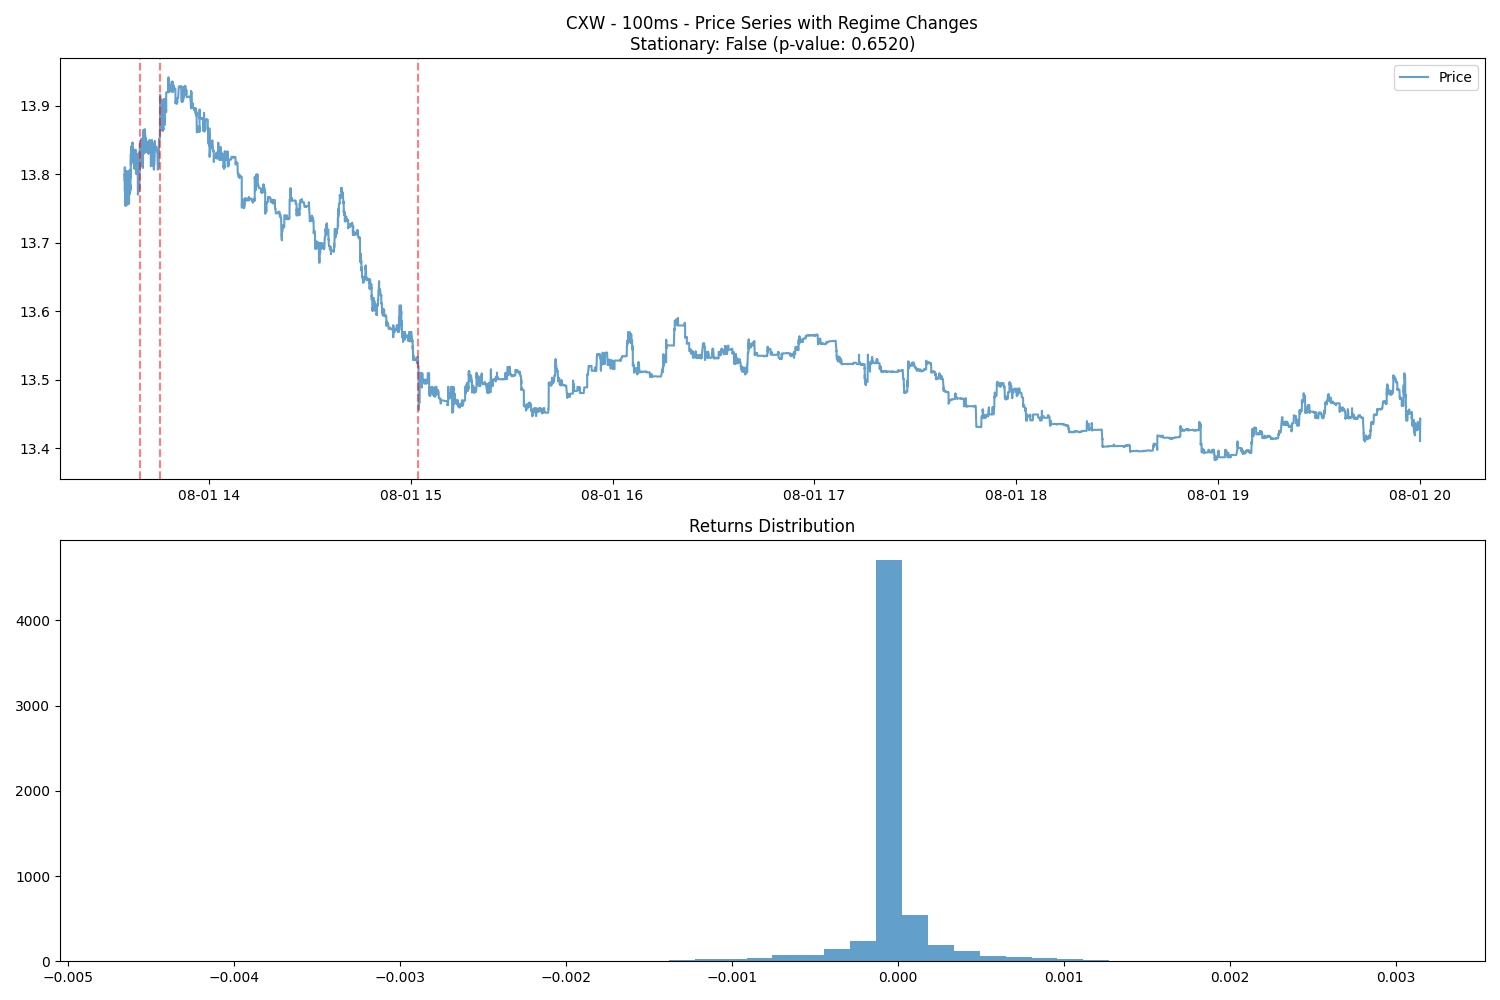
\includegraphics[width=0.45\textwidth]{results/stationarity/stats/CXW/CXW_2024-08-01_100ms.png}
    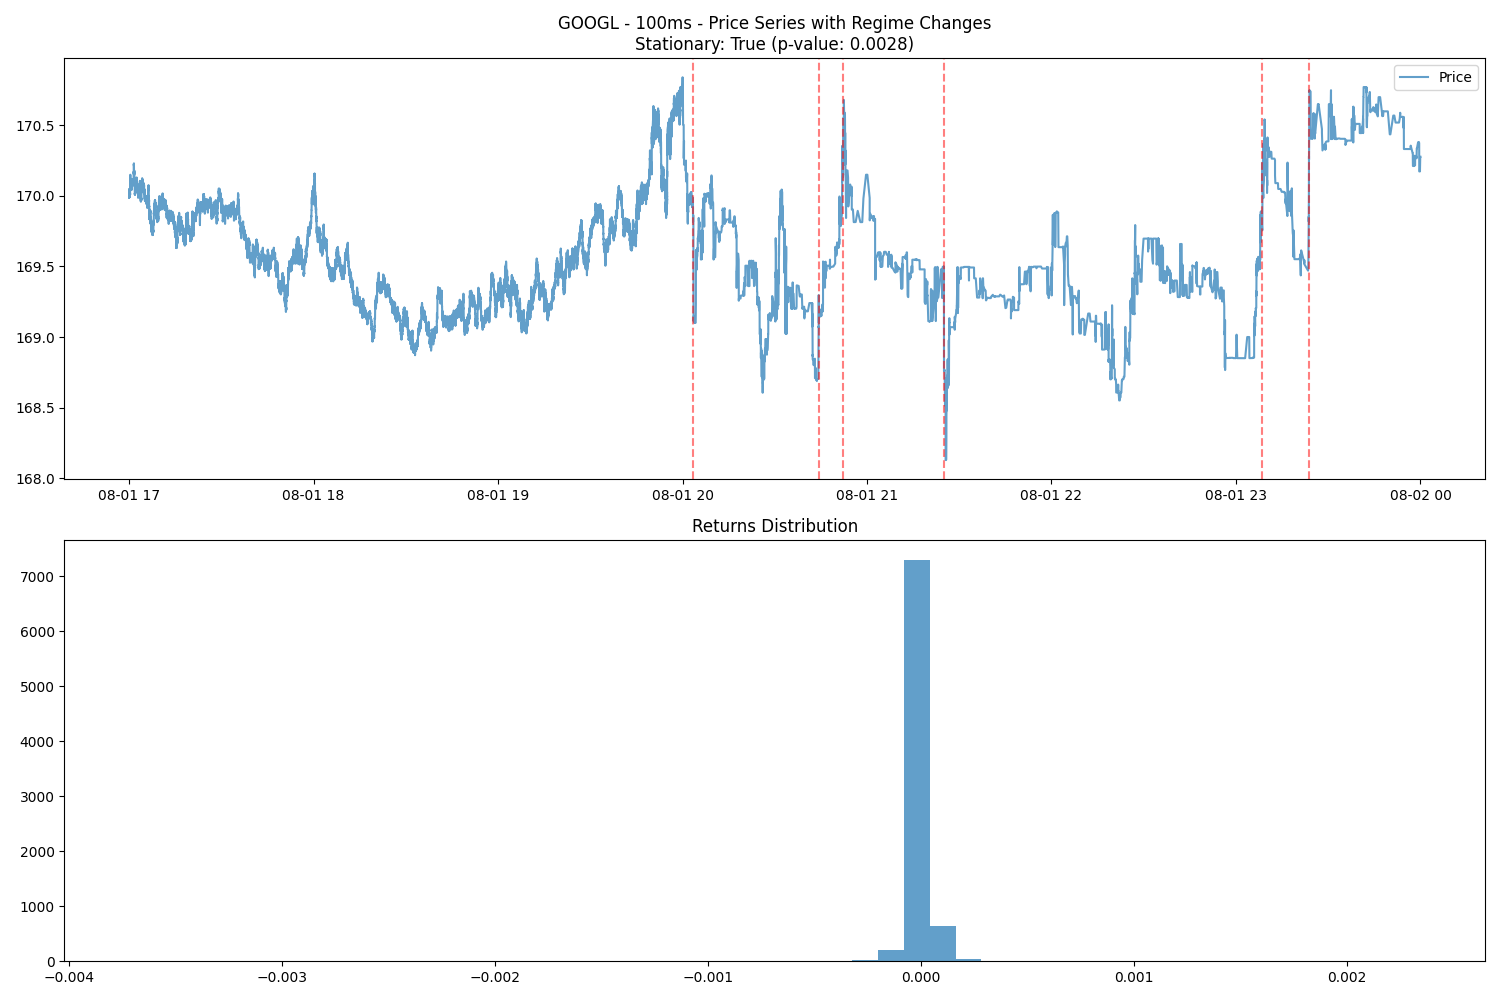
\includegraphics[width=0.45\textwidth]{results/stationarity/stats/GOOGL/GOOGL_2024-08-01_100ms.png}
    \caption{Analyse de stationnarité pour INTC, AAL, CXW et GOOGL le 8 août 2024 à l'échelle de 100ms. Les lignes verticales rouges indiquent les changements de régime détectés.}
    \label{fig:stationarity_unemployment}
\end{figure}

Cette journée met en évidence plusieurs phénomènes importants :

\begin{itemize}
    \item \textbf{Synchronisation des ruptures} : Les quatre actifs présentent des changements de régime simultanés au moment de l'annonce (14:30 GMT), malgré leurs secteurs d'activité différents.
    
    \item \textbf{Impact sur les corrélations} : Bien que l'événement affecte tous les actifs, son effet disparaît dans l'analyse des copules car :
    \begin{itemize}
        \item La normalisation par la moyenne journalière élimine l'effet de niveau commun
        \item Les rendements sont calculés après suppression de la tendance locale
        \item Les changements de régime sont traités comme des points de rupture distincts
    \end{itemize}
    
    \item \textbf{Échelles multiples} : L'impact est visible différemment selon l'échelle d'observation :
    \begin{itemize}
        \item À 100ms : Rupture nette et synchronisée
        \item À 1s : Persistance de l'effet avec retour progressif à la normale
        \item À 60s : Intégration de l'information dans un nouveau régime stable
    \end{itemize}
\end{itemize}

Cette observation est fondamentale car elle démontre que l'apparente indépendance des rendements à haute fréquence n'est pas incompatible avec l'existence de mouvements coordonnés du marché. La stationnarité locale est préservée précisément parce que ces événements sont traités comme des points de rupture plutôt que comme des variations continues du processus.

\subsubsection{Synthèse des analyses de dépendance et stationnarité}

L'analyse conjointe des copules et de la stationnarité nous permet de tirer plusieurs conclusions importantes sur la nature des dépendances dans les marchés haute fréquence :

\begin{itemize}
    \item Les séries temporelles présentent une indépendance conditionnelle forte à l'échelle microscopique, confirmée par la faiblesse des dépendances capturées par les copules à ces échelles ($\tau < 0.2$ pour $\Delta t < 1\text{ms}$).
    
    \item Les changements de régime majeurs sont synchronisés entre les différents actifs, comme observé notamment lors de l'annonce des taux de la Fed le 18 septembre 2024, suggérant une source commune de non-stationnarité.
    
    \item La structure de dépendance évolue avec l'échelle temporelle : alors que les prix sont largement indépendants à l'échelle microscopique, des motifs de dépendance plus forts émergent aux échelles plus longues, particulièrement en période de stress.
\end{itemize}

Ces résultats soulignent l'importance d'une approche multi-échelle dans l'analyse des marchés haute fréquence, où les propriétés statistiques des séries de prix varient significativement selon l'horizon temporel considéré.

\begin{figure}[h!]
    \centering
    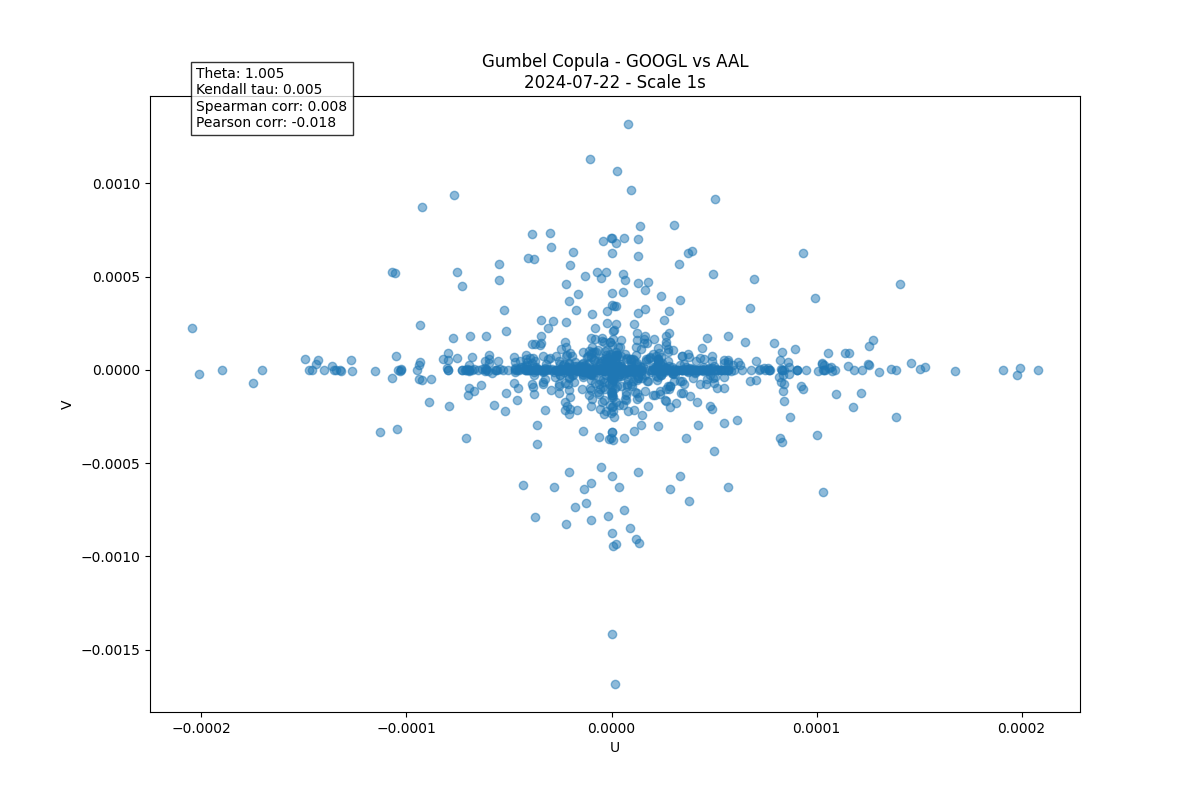
\includegraphics[width=0.8\textwidth]{results/copulas/GOOGL_AAL_2024-07-22_1s.png}
    \caption{Copule de Gumbel estimée pour la paire GOOGL-AAL le 22 juillet 2024 à l'échelle 1s. Les paramètres estimés montrent une faible dépendance ($\theta = 1.005$, $\tau = 0.005$), cohérente avec l'hypothèse d'indépendance conditionnelle à haute fréquence.}
    \label{fig:copula_example}
\end{figure}

\end{document}